\chapter{Diagonalization}
\Opensolutionfile{solutions}[solutions/diagonalization]

A basic goal of complexity theory is to prove that certain complexity classes (e.g. $\PTIME$ and $\NPTIME$) are not the same. To do so, we need to exhibit a machine in one class that differs from every machine in other class in the sense that their answers are different on at least one input. This chapter describes \vocab{diagonalization}—essentially the only general technique known for constructing such a machine.

In this chapter, we will use diagonalization in clever ways. We first use it in \secref{time-hierarchy-theorem} and \secref{nondeterministic-time-hierarchy-theorem} to prove hierarchy theorems, which show that giving Turing machines more computational resources allows them to solve a strictly larger number of problems. We then use diagonalization in \secref{ladner-theorem} to show a fascinating theorem of Ladner: If $\PTIME \neq \NPTIME$, then there exists a problem that are neither $\NPTIME$-complete nor in $\PTIME$.

Though diagonalization led to some of these early successes of complexity theory, researchers concluded in the 1970s that diagonalization alone may not resolve $\PTIME$ vs $\NPTIME$ and other interesting questions. \secref{oracle-machines-and-the-limits-of-diagonalization} describes their reasoning. Ironically, these limits of diagonalization are proved using diagonalization itself.

\section{Time Hierarchy Theorem}
\seclabel{time-hierarchy-theorem}
Common sense suggests that giving a Turing machine more time should increase the class of problems that it can solve. For example, Turing machines should be able to decide more languages in time $n^3$ than they can in $n^2$. The \vocab{time hierarchy theorem} proves that this intuition is correct, subject to certain conditions described below. We use the term ``hierarchy theorem'' because this theorem proves that time complexity classes aren't all the same—they form a hierarchy whereby the classes with larger bounds contain more languages than the classes with smaller bounds.

We begin with the following technical definition, given by Goldreich \cite{goldreich2008computational}.

\begin{definition}[Time-constructible functions]
  A function $f : \NN \to \NN$ is called \vocab{time-constructible} if there exists a TM $M$ which, given a string $\texttt{1}^n$, outputs the binary representation of $f(n)$ in $O(f(n))$ time.
\end{definition}

\begin{example}
  All the commonly used functions $f(n)$ are time-constructible, as long as $f(n)$ is at least $c \cdot n$ for some constant $c > 0$. No function which is $o(n)$ can be time-constructible unless it is eventually constant, since there is insufficient time to read the entire input.
\end{example}

When designing algorithms of arbitrary time complexity $f : \NN \to \NN$, we need to make sure that the algorithm does not exceed the time bound. However, when invoked on an input $w$, we cannot assume that the algorithm is given the time bound $f(\len{w})$ explicitly. A reasonable design methodology is to have the algorithm compute this bound before doing anything else. This, in turn, requires the algorithm to read the entire input and compute $f(n)$ in $O(f(n))$ steps; otherwise, this preliminary stage already consumes too much time. The latter requirement motivates the notion of time-constructible functions.

There are multiple definitions of the time hierarchy theorem. We present the following one by Sipser \cite{sipser2013introduction}, with some correction.

\begin{theorem}[Time hierarchy theorem]
  \thmlabel{time-hierarchy-theorem}
  For any time-constructible function $f : \NN \to \NN$ where $f(n) = \omega(n \log n)$, a language $A$ exists that is decidable in $O(f(n))$ time but not decidable in time $o(f(n) / \log f(n))$.
\end{theorem}

We present the following proof by Sipser \cite{sipser2013introduction}, with some modification.

\begin{proofidea}
  We must demonstrate a language $A$ that has two properties. The first says that $A$ is decidable in $O(f(n))$ time. The second says that $A$ isn't decidable in $o(f(n) / \log f(n))$ time.

  We describe $A$ by giving an algorithm $D$ that decides it. Algorithm $D$ runs in $O(f(n))$ time, thereby ensuring the first property. Furthermore, $D$ guarantees that $A$ is different from any language that is decidable in $o(f(n) / \log f(n))$ time, thereby ensuring the second property. Notice that language $A$ is different from other languages in that it lacks a non-algorithmic definition. Therefore, we cannot offer a simple mental picture of $A$.

  In order to ensure that $A$ is not decidable in $o(f(n) / \log f(n))$ time, we design $D$ to implement the diagonalization method. If $M$ is a TM that decides a language in $o(f(n) / \log f(n))$ time, $D$ guarantees that $A$ differs from $M$'s language in at least one place. Which place? The place corresponding to a description of $M$ itself.

  Let's look at the way $D$ operates. Roughly speaking, $D$ takes its input to be the description of a TM $M$. (If the input isn't the description of any TM, then $D$'s action is inconsequential on this input, so we arbitrarily make $D$ reject.) Then, $D$ runs $M$ on the same input—namely, $\enc{M}$—within the time bound $\ceil{f(n) / \log f(n)}$. If $M$ halts within that much time, $D$ accepts iff $M$ rejects. If $M$ doesn't halt, $D$ just rejects. So if $M$ runs within time $\ceil{f(n) / \log f(n)}$, $D$ has enough time to ensure that its language is different from $M$'s. If not, $D$ doesn't have enough time to figure out what $M$ does, but fortunately $D$ has no requirement to act differently from machines that don't run in $o(f(n) / \log f(n))$ time, so $D$'s action on this input is inconsequential.

  This description captures the essence of the proof but omits several important details. If $M$ runs in $o(f(n) / \log f(n))$ time, $D$ must guarantee that its language is different from $M$'s language. But even when $M$ runs in $o(f(n) / \log f(n))$ time, it may use more than $f(n)$ time for small $n$, when the asymptotic behavior hasn't ``kicked in'' yet. Possibly, $D$ might not have enough time to run $M$ to completion on the input $\enc{M}$, and hence $D$ will miss its opportunity to avoid $M$'s language. So, if we aren't careful, $D$ might end up deciding the same language $M$ decides, and the theorem wouldn't be proved.

  We can fix this problem by modifying $D$ to give it additional opportunities to avoid $M$'s language. Instead of running $M$ only when $D$ receives the input $\enc{M}$, it runs $M$ whenever it receives an input of the form $\enc{M}\texttt{1}\texttt{0}^\ast$, that is, an input of the form $\enc{M}$ followed by a $\texttt{1}$ and some number of $\texttt{0}$s. Observe that by doing this, we get to simulate $M$ on infinitely many $w$, so now $D$ has infinitely many opportunities to avoid $M$'s language. Then, if $M$ really is running in $o(f(n) / \log f(n))$, we will eventually encounter a sufficiently large $w$, where $w = \enc{M}\texttt{1}\texttt{0}^k$ for some large value of $k$, and $D$ will have enough time to run it to completion because the asymptotic must eventually kick in.

  One last technical point. The simulation of $M$ by $D$ introduces a logarithmic factor overhead. This overhead is the reason for the appearance of the $1 / \log f(n)$ factor in the statement of this theorem. If we had a way of simulating a single-tape TM by another single-tape TM for a prespecified number of steps, using only a constant factor overhead in time, we would be able to strengthen this theorem by changing $o(f(n) / \log f(n))$ to $o(f(n))$. No such efficient simulation is known.
\end{proofidea}

We now describe the proof formally.

\begin{proof}
  The following $O(f(n))$ time algorithm $D$ decides a language $A$ that is not decidable in $o(f(n) / \log f(n))$ time.

  \begin{turing}{$D$}{On input $w$:}
  \item If $w$ is not of the form $\enc{M}\texttt{1}\texttt{0}^\ast$ for some TM $M$, \emph{reject}.
  \item Let $n$ be the length of $w$.
  \item Compute $f(n)$ using time constructibility, and store the value $\ceil{f(n) / \log f(n)}$ in a binary counter. Decrement this counter before each step used to carry out stage 4. If the counter ever hits 0, \emph{reject}.
  \item Simulate $M$ on $w$.
  \item If $M$ accepts, then \emph{reject}. If $M$ rejects, then \emph{accept}.
  \end{turing}

  We examine each of the stages of this algorithm to determine the running time. Obviously, stages 1, 2, and 3 can be performed within $O(f(n))$ time. In stage 4, every time $D$ simulates one step of $M$, it takes $M$'s current state together with the tape symbol under $M$'s tape head and looks up $M$'s next action in its transition function so that it can update $M$'s tape appropriately. All three of these objects (state, tape symbol, and transition function) are stored on $D$'s tape somewhere. If they are stored far from each other, $D$ will need many steps to gather this information each time it simulates one of $M$'s steps. Instead, $D$ always keep this information close together.

  We can think of $D$'s single tape as organized into \emph{tracks}. One way to get two tracks is by storing one track in the odd positions and the other in the even positions. Alternatively, the two-track effect may be obtained by enlarging $D$'s tape alphabet to include each pair of symbols, one from the top track and the second from the bottom track. We can get the effect of additional tracks similarly. Note that multiple tracks introduce only a constant factor overhead in time, provided that only a fixed number of tracks are used. Here, D has three tracks.

  One of the tracks contains the information on $M$'s tape, and a second contains its current state and a copy of $M$'s transition function. During the simulation, $D$ keeps the information on the second track near the current position of $M$'s head on the first track. Every time $M$'s head position moves, $D$ shifts all the information on the second track to keep it near the head. Because the size of the information on the second track depends only on $M$ and not on the length of the input to $M$, the shifting adds only a constant factor to the simulation time. Furthermore, because the required information is kept close together, the cost of looking up $M$'s next action in its transition function and updating its tape is only a constant. Hence, if $M$ runs in $g(n)$ time, $D$ can simulate it in $O(g(n))$ time.

  At every step in stage 4, $D$ must decrement the step counter originally set in stage 3. Here, $D$ can do so without adding excessively to the simulation time by keeping the counter in binary on a third track and moving it to keep it near the present head position. This counter has a magnitude of about $f(n) / \log f(n)$, so its length is $\log(f(n) / \log f(n))$, which is $O(\log f(n))$. Hence, the cost of updating and moving at each step adds a $\log f(n)$ factor to the simulation time, thus brining the total running time to $O(f(n))$. Therefore, $A$ is decidable in time $O(f(n))$.

  Now, we show that $A$ is not decidable in $o(f(n) / \log f(n))$ time. Assume the contrary that some TM $M$ decides $A$ in time $g(n)$, where $g(n)$ is $o(f(n) / \log f(n))$. Here, $D$ can simulate $M$, using time $d \cdot g(n)$ for some constant $d$. If the total simulation time (not counting the time to update the step counter) is at most $f(n) / \log f(n)$, the simulation will run to completion. Because $g(n)$ is $o(f(n) / \log f(n))$, some constant $n_0$ exists where $d \cdot g(n) < f(n) / \log f(n)$ for all $n \geq n_0$. Therefore, $D$'s simulation of $M$ will run to completion as long as the input has length $n_0$ or more. Consider what happens when we run $D$ on the input $\enc{M}\texttt{1}\texttt{0}^{n_0}$. This input is longer than $n_0$ so the simulation in stage 4 will complete. Therefore, $D$ will do the opposite of $M$ on the same input. Hence, $M$ doesn't decide $A$, which contradicts our assumption. Therefore, $A$ is not decidable in $o(f(n) / \log f(n))$ time.
\end{proof}

\begin{remark}
  Actually, there is one other technical detail that we conveniently ignored in our proof, in order to keep it concise. Let us discuss the detail here. In Stage $4$ of $D$, it simulates $M$ on $w$. This simulation may require representing each cell of $M$'s tape with several cells on $D$'s tape because $M$'s tape alphabet is arbitrary while D's tape alphabet is fixed. However, initializing the simulation by converting $D$'s input $w$ to this representation involves rewriting $w$ so that its symbol are spread apart by several cells. Let $n$ be the length of $w$. If we use the obvious copying procedure for spreading $w$, this convention would involve $O(n^2)$ time and that would exceed the $O(f(n))$ time bound for small $f$. Instead, we observe that $D$ operates on an input $w$ of the form $\enc{M}\texttt{1}\texttt{0}^k$, and we only need to carry out the simulation when $k$ is sufficiently large. We consider only $k > \len{\enc{M}}^2$. We can spread out $w$ by first using the obvious copying procedure for $\enc{M}$ and then counting the trailing $\texttt{0}$s and rewriting these by using that count. The time for spreading $\enc{M}$ is $O(\len{\enc{M}}^2)$ which is $O(n)$. The time for counting the $\texttt{0}$s is $O(n \log n)$, which is $O(f(n))$.
\end{remark}

\begin{remark}
  We also didn't elaborate on the fact that our function $f(n)$ is $\omega(n \log n)$ in the statement of our theorem. This is because, as we will demonstrate in \corref{alternative-definition-of-time-hierarchy-theorem}, the time hierarchy theorem can be used to distinguish between two complexity classes, e.g. $\DTIME(f(n))$ and $\DTIME(g(n))$. We require both functions $f$ and $g$ to be time-constructible.
\end{remark}

\begin{remark}
  Hartmanis and Stearns \cite{hartmanis1965computational} were the first to establish the time hierarchy theorem. A year later, Hennie and Stearns \cite{hennie1966two} improved this result by demonstrating that $t$ steps on any $k$-tape TM can be simulated in $O(t \log t)$ steps on a two-tape TM. Although we managed to obtain an equally sharp time hierarchy, it's worth noting that we proved our theorem by simulating a single-tape TM with another single-tape TM. This specific approach was originally established by Hartmanis and Hopcroft \cite{hartmanis1968computational}. Curiously, their original proof did not rely solely on simulation; it distinguished between two cases:
  \begin{enumerate}
    \item When the running time is $\Omega(n^2)$, simulation is used, much like what we did in our proof.
    \item \dubious{When the running time is $o(n^2)$, they presented a language directly for the separation, without using simulation. This part of the proof depended on specific properties of single-tape TMs with sub-quadratic running times.}
  \end{enumerate}
\end{remark}
\todo{Verify this. Also clarify whose running time? The machine simulating or simulated?}

Now we can introduce the following important corollary, which is very frequently referred to as the time hierarchy theorem in other literature.

\begin{corollary}
  \corlabel{alternative-definition-of-time-hierarchy-theorem}
  For any two time-constructible functions $f, g : \NN \to \NN$ where $f(n) \log f(n) = o(g(n))$,
  \[ \DTIME(f(n)) \subsetneq \DTIME(g(n)). \]
\end{corollary}

This corollary allows us to separate various deterministic time complexity classes. For example, we can show that the function $n^c$ is time-constructible for any natural number $c$. Hence, for any two natural numbers $c_1 < c_2$ we can prove that $\DTIME(n^{c_1}) \subsetneq \DTIME(n^{c_2})$. With a bit more work we can show that $n^c$ is time-constructible for any rational number $c > 1$ and thereby extend the preceding containment to hold for any rational numbers $1 \leq c_1 < c_2$. Observing that two rational numbers $c_1$ and $c_2$ always exist between any two real numbers $\epsilon_1 < \epsilon_2$ such that $\epsilon_1 < c_1 < c_2 < \epsilon_2$ we obtain the following additional corollary demonstrating a fine hierarchy within the class $\PTIME$.

\begin{corollary}
  \corlabel{time-hierarchy-theorem-for-the-class-P}
  For any two real numbers $1 \leq \epsilon_1 < \epsilon_2$,
  \[ \DTIME(n^{\epsilon_1}) \subsetneq \DTIME(n^{\epsilon_2}). \]
\end{corollary}

We can also use the time hierarchy theorem to separate the classes $\PTIME$ and $\EXPTIME$.

\begin{corollary}
  \corlabel{ptime-strict-subset-of-exptime}
  $\PTIME \subsetneq \EXPTIME$.
\end{corollary}

\begin{proof}
  We have
  \[ \DTIME(2^n) \subseteq \DTIME\left(o\left(\frac{2^{2n}}{2n}\right)\right) \subsetneq \DTIME(2^{2n}) \]
  by the time hierarchy theorem. It follows that
  \[ \PTIME \subseteq \DTIME(2^n) \subsetneq \DTIME(2^{2n}) \subseteq \EXPTIME. \]
\end{proof}

This corollary establishes the existence of decidable problems that are decidable in principle but not in practice—that is, problems that are decidable but intractable.

\begin{remark}
  In fact, we can show that $\PTIME$ is strictly contained within $\EXPTIME$ without explicitly relying on the time hierarchy theorem. Instead, we'll provide a direct proof using—you guessed it—diagonalization!

  \begin{proof}
    Let
    \[ L = \set{(\enc{M}, x, \texttt{1}^n) \mid \text{$M(x)$ halts in at most $2^n$ steps}}. \]
    Clearly $L \in \EXPTIME$. On the other hand, suppose by contradiction that $L \in \PTIME$. Then there's some polynomial-time Turing machine $A$ such that $A(w)$ accepts if and only if $w \in L$. Let $A$ runs in $p(n + \len{\enc{M}} + \len{x})$ on input $(\enc{M}, x, \texttt{1}^n)$, for some polynomial function $p$. Then using $A$, we can easily produce another machine $B$ that does the following.

    \begin{turing}{$B$}{On input $w = (\enc{M}, \texttt{1}^n)$:}
    \item Use $A$ to decide if $M(\enc{M}, \texttt{1}^n)$ halts in at most $2^n$ steps.
    \item If it does, run forever.
    \item Otherwise, halt.
    \end{turing}

    Note that, if $B$ halts at all, then it halts after only $p(2n + 2 \enc{M}) = n^{O(1)}$ steps. Now consider what happens when $B$ is run on input $(\enc{B}, \texttt{1}^n)$. If $B(\enc{B}, \texttt{1}^n)$ runs forever, then $B(\enc{B}, \texttt{1}^n)$ halts. Conversely, if $B(\enc{B}, \texttt{1}^n)$ halts, then for all sufficiently large $n$, it halts in fewer than $2^n$ steps, but that means that $B(\enc{B}, \texttt{1}^n)$ runs forever. So we conclude that $B$, and hence $A$, cannot exist.
  \end{proof}
\end{remark}

\section{Nondeterministic Time Hierarchy Theorem}
\seclabel{nondeterministic-time-hierarchy-theorem}
The time hierarchy theorem for nondeterministic Turing machines was originally proven by Cook \cite{cook1972hierarchy}. The following tighter result is due to Seiferas, Fischer, and Meyer \cite{seiferas1978separating}.

\begin{theorem}[Nondeterministic time hierarchy theorem]
  For any two time-constructible functions $f, g : \NN \to \NN$ where $f(n + 1) = o(g(n))$,
  \[ \NTIME(f(n)) \subsetneq \NTIME(g(n)). \]
\end{theorem}

\begin{remark}
  The effect of the term ``$+ 1$'' in $f(n + 1)$ is pretty significant. Specifically, it makes a difference to all time-constructible function $t : \NN \to \NN$ where $t(n) = \omega(2^n)$. For instance, consider the functions $f_1(n) = 2^{n^2}$ and $f_2(n) = 2^{(n + 1)^2}$. Our hierarchy theorem is not sharp enough to separate the classes $\NTIME(f_1(n))$ and $\NTIME(f_2(n))$, because $f_1(n + 1) \neq o(f_2(n))$.
\end{remark}

Our first instinct is to duplicate the proof of \thmref{time-hierarchy-theorem}, since there is a universal TM for nondeterministic computation as well. (In fact, the simulation of an NTM by another NTM is very efficient, incurring only a constant factor overhead in time \cite{arora2009computational}.) The problem, however, is that we don't know how such a construction would work on our new machine $D$. In particular, it remains unclear how we could ``flip the answer'' of $M$—to \emph{efficiently} compute, given the description of an NTM $M$ and an input $w$, the value $1 - M(w)$. We give the following hypothetical (erroneous) construction of $D$ to illustrate our point.

\begin{turing}{$D$}{On input $w$:}
\item Let $n$ be the length of $w$.
\item If $w$ is not of the form $\enc{M}\texttt{1}\texttt{0}^\ast$ for some TM $M$, \emph{reject}.
\item Nondeterministically simulate $M$ on $w$ for up to $g(n)$ steps.
  \begin{enumerate}[label=\theenumi\arabic*.]
    \item If $M$ accepts, then \emph{reject}.
    \item \incorrect{If $M$ rejects, then \emph{accept}. (How to decide this efficiently so the simulation does not timeout?)}
  \end{enumerate}
\end{turing}

A nondeterministic Turing machine accepts if at least one path accepts; it rejects only when \emph{all paths reject}. This asymmetry makes it hard to flip answers efficiently. For instance, suppose we have an NTM $M$ that has two paths for input $w$ where one accepts and the other rejects. $M$ has at least one accepting path for $w$, so it accepts. Suppose we want to produce a machine that accepts exactly the input that $M$ rejects. The obvious attempt is to take $M$ and make its accepting state reject, and its rejecting states accept. However, this new machine $M'$ has one rejecting path and one accepting path. So it still accepts $w$, which it was supposed to reject.

One limitation of the nondeterministic Turing machine is that it can't look at all its paths simultaneously and take action based on what all of those paths do. When simulating an NTM $M$ with another machine $M'$, each path $M'$ can only simulate one path of $M$ and has no knowledge of the other paths. It cannot decide to accept/reject based on the outcomes of paths it cannot see. Therefore, each path of $M'$ can only follow simple rules based on its own outcome. When $M'$ discovers that $M$ rejects the input $w$ on a certain path, $M'$ still \emph{cannot} verify whether $w$ is in the language of $M$ or not (because of the asymmetric accept/reject condition of the NTM). Therefore, it seems that the only reliable way to determine if $M$ rejects $w$ is to exhaustively check every possible path, which is exponentially more time-consuming than checking a single path.

What now? There are two options here:
\begin{enumerate}
  \item We admit defeat. Accept the exponential-time slowdown, but then we won't get a fine hierarchy at all.
  \item Or, we try to come up with a better solution. Consider the following idea. Now, our new simulator is in no hurry to diagonalize, it will not try to flip the answer of a subroutine NTM on every input, but only on a crucial input out of a sufficiently large interval. This technique is known as \vocab{lazy diagonalization}. We show that it does suffice to establish our hierarchy theorem.
\end{enumerate}

We present the following proof, inspired by Žák \cite{zak1983turing}.

\begin{proofidea}
  Recall that in our proof of the deterministic time hierarchy theorem, $D$ gets to simulate $M$ infinitely often. When the input strings get long enough, $D$ accepts iff $M$ rejects. This means that $D$ exhibits different behavior from $M$ on infinitely many inputs. This diagonalization technique demonstrates that no other TM $M$ (that is significantly more efficient than $D$) can accept the same language as $D$. However, observe that this is somewhat redundant. That is, $D$ does \emph{not} need to diverge from $M$ infinitely often. In fact, we only need $D$ to behave differently at least once, and our proof would have still held. This is the essence of lazy diagonalization and represents our first key observation for our proof of the nondeterministic time hierarchy theorem.

  Next, our second key observation comes from the fact that we can ``feed'' $M$ with an input that is much smaller than the original input. When $D$ receives the input $\texttt{1}^n$, rather than simulating $M$ on $\texttt{1}^n$, we can opt to simulate an exponentially smaller input, say $\texttt{1}^{\log n}$, on $M$ instead. Why would we want to do this? Currently, we have no effective means of deciding if $M$ rejects some input $w$. Our only reliable strategy for now is to exhaustively check every computation path of $M$. But $M$ may have exponentially many such paths. (Recall that this was the main roadblock that we faced earlier.) Consider what happens when we simulate $\texttt{1}^{\log n}$ on $M$. If simulating one path of $M$ takes $\len{\texttt{1}^{\log n}} = O(\log n)$ time, then simulating all computation paths would require $2^{O(\log n)}$ time, which is $\poly(n)$. Notice that $\poly(n)$ is polynomial in the length of our original input string $\texttt{1}^n$. This means that $D$ won't run out of time while simulating $M$!

  The set of all Turing machines is enumerable. Let $M_k$ be the $k$-th Turing machine in the enumeration. We can associate each TM $M_k$ with an interval $I_k = (l_k, u_k]$ (of natural numbers, i.e. $\NN$). These intervals should be disjoint but contiguous. Each interval $I_k$ is large, so we get to simulate $M_k$ on a lot of input words. Crucially, the upper bound of the interval, $u_k$, should at the very least be exponentially larger than the lower bound, $l_k$.

  Here's where the magic happens. Consider what happens when we run $D$ on all the inputs that correspond to a single interval $I_k = (l_k, u_k]$ (thus, a single TM $M_k$). When $D$ receives the input $\texttt{1}^n$ where $n < u_k$, $D$ accepts $\texttt{1}^n$ iff $M_k$ accepts $\texttt{1}^{n + 1}$. Here, we refrain ourselves from diagonalizing. However, when $D$ receives the input $\texttt{1}^n$ where $n = u_k$, we diagonalize but on a much smaller input, i.e. $D$ accepts $\texttt{1}^n$ iff $M_k$ rejects $\texttt{1}^{l_k + 1}$. In this case, $D$ has sufficient time to simulate $M_k$ as we have established earlier. Furthermore, we have effectively demonstrated that no TM $M_k$ can accept the same language as $D$, since $D$ diverge from $M_k$ on exactly one input, i.e. on the input $\texttt{1}^n$ where $n = u_k$. To further illustrate this fact, consider the following graphical representation of an equivalence class and a non-equivalence relation that we obtain, by virtue of our construction.
  \begin{center}
    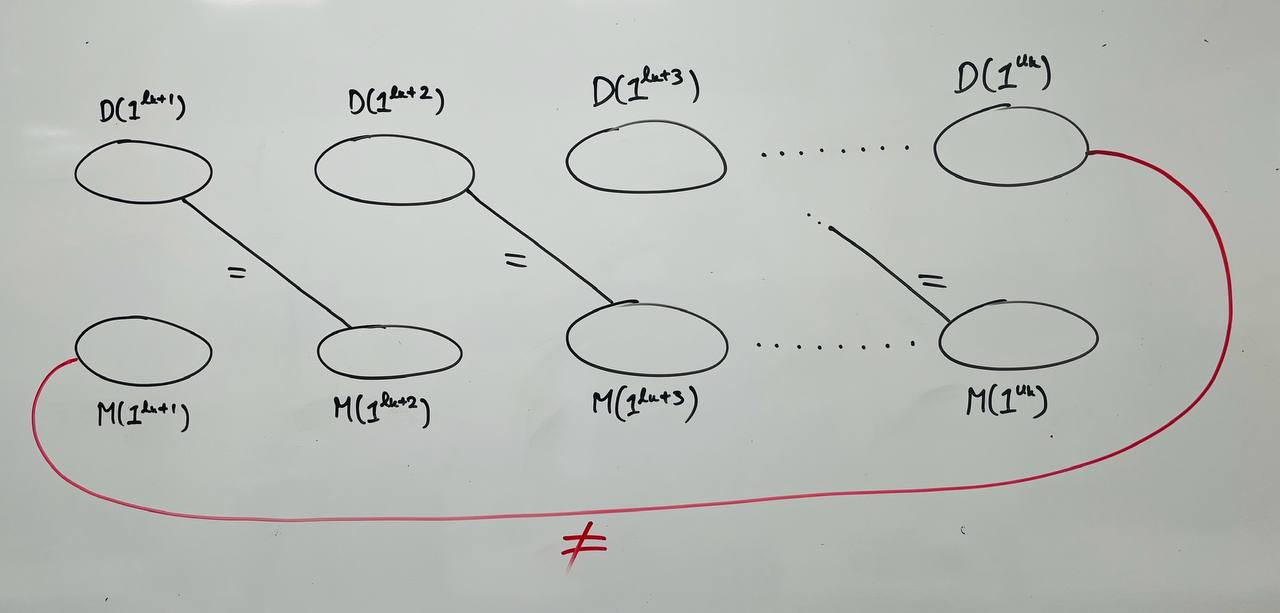
\includegraphics[width=0.75\textwidth]{media/lazy_diagonalization.jpg}
  \end{center}
  If we assume the contrary that $M_k$ accepts the same language as $D$, then we get the following new equivalence class.
  \begin{center}
    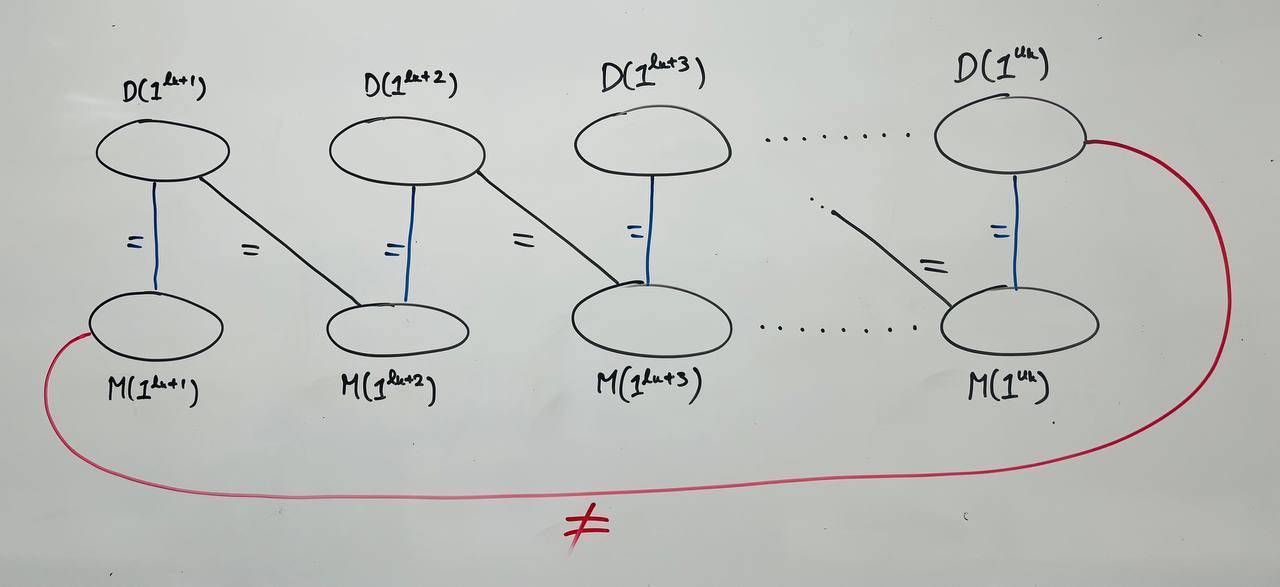
\includegraphics[width=0.75\textwidth]{media/lazy_diagonalization_contradiction.jpg}
  \end{center}
  This means that we have $M(\texttt{1}^{l_k + 1}) = D(\texttt{1}^{u_k})$ by $\relbar\!\relbar\!\relbar$ and \textcolor{blue}{$\relbar\!\relbar\!\relbar$}, but $M(\texttt{1}^{l_k + 1}) \neq D(\texttt{1}^{u_k})$ by \textcolor{red}{$\relbar\!\relbar\!\relbar$}. A contradiction.

  One last technical point. Just as in the proof of the deterministic time hierarchy theorem, we may encounter a similar issue where the asymptotic behavior of $f$ has not yet taken effect. To fix this problem, it suffices to simply restrict the simulation of $D$ on sufficiently long inputs. We then associate the first(s) of these inputs to the first interval, $I_1$.
\end{proofidea}

Now, we describe the proof formally.

\begin{proof}
  We know that the set of all Turing machines is enumerable. Let $M_k$ be the $k$-th Turing machine in the enumeration. We associate $M_k$ with an interval $I_k = (l_k, u_k]$, where $f(u_k) > 2^{f(l_k + 1)^2}$. These intervals should be disjoint but contiguous. Because $f(n + 1)$ is $o(g(n))$, some constant $n_0$ exists where $d \cdot f(n + 1) < g(n)$ for all $n \geq n_0$. We set the lower bound of the first interval $l_1$, to $n_0$. Our NTM $D$ will try to flip the answer of $M_k$ only on one input in the interval $I_k$. We define $D$ as follows:

  \begin{turing}{$D$}{On input $w$:}
  \item Let $n$ be the length of $w$.
  \item If $w$ is not of the form $\texttt{1}^n$ where $n \geq n_0$, \emph{reject}.
  \item Compute $k$ such that $n$ lies in the interval $I_k = (l_k, u_k]$.
    \begin{enumerate}[label=\theenumi\arabic*.]
      \item If $n < u_k$, then nondeterministically simulate $M_k$ on the input $\texttt{1}^{n + 1}$ for up to $g(n)$ steps. If $M$ accepts, then \emph{accept}. If $M$ rejects, then \emph{reject}. (Observe that here we are \emph{not} diagonalizing.)
      \item If $n = u_k$, then deterministically decide if $M_k$ accepts the input $\texttt{1}^{l_k + 1}$ by simulating all computation paths, for up to $g(n)$ steps in total. If $M$ accepts, then \emph{reject}. If $M$ rejects, then \emph{accept}. (Observe that here we are \emph{indeed} diagonalizing. But we are doing it on a much shorter input than the input to $D$.)
    \end{enumerate}
  \end{turing}

  Let's analyze the running time of each stage of $D$. Stage 1 and 2 clearly operate in $O(g(n))$ time. Stage 3 can also be performed in $O(g(n))$ time, since $k \ll n$. In stage 3.1, $D$ nondeterministically simulates $M_k$ on the input $\texttt{1}^{n + 1}$. If $M_k$ really runs within $O(f(n + 1))$ time, then $D$ has sufficient time for the simulation, since $f(n + 1) = o(g(n))$. Otherwise, if $M_k$ doesn't halt, $D$ will terminate the simulation after $g(n)$ steps. In both cases, $D$ runs within $O(g(n))$ time. In stage 3.2, $D$ deterministically simulates every computation path of $M_k$ on the input $\texttt{1}^{l_k + 1}$. If $M_k$ really runs within $O(f(l_k + 1))$, $D$ again has sufficient time for the simulation. The deterministic simulation of each computation path requires $O(f(l_k + 1) \log f(l_k + 1))$, leading to a total time for all paths of $2^{O(f(l_k + 1) \log f(l_k + 1))}$. This is less than $2^{f(l_k + 1)^2} < f(u_k) = f(n) = o(g(n))$. Otherwise, if $M_k$ doesn't halt, $D$ will stop the simulation after $g(n)$ steps. In both cases, $D$ runs within $O(g(n))$ time.

  Now, we show that $A$ is not decidable in $O(f(n))$ time. Assume the contrary that some TM $M_k$ decides $A$ in time $f(n)$, where $f(n + 1)$ is $o(g(n))$. Here, $D$ can simulate $M_k$, using time $d \cdot g(n)$ for some constant $d$. Because $f(n + 1)$ is $o(g(n))$, some constant $n_0$ exists where $d \cdot f(n + 1) < g(n)$ for all $n \geq n_0$. Therefore, $D$'s simulation of $M_k$ will run to completion as long as the input has length $n_0$ or more. Consider what happens when we run $D$ on all the inputs $\texttt{1}^n$ where $n \geq n_0$, such that all these inputs correspond to the interval $I_k = (l_k, u_k]$. Stages 3.1 and 3.2 of $D$ ensure, respectively, that:
  \begin{align}
    \text{$M_k(\texttt{1}^{n + 1}) = D(\texttt{1}^n)$} & \qquad \text{if $l_k < n < u_k$} \\
    \text{$M_k(\texttt{1}^{l_k + 1}) \neq D(\texttt{1}^{u_k}) = D(\texttt{1}^n)$} & \qquad \text{if $n = u_k$}
  \end{align}
  By our assumption, $D$ and $M_k$ agree on all inputs $\texttt{1}^n$ in the interval $I_k = (l_k, u_k]$. Together with (2.1), this implies $M(\texttt{1}^{l_k + 1}) = D(\texttt{1}^{l_k + 1}) = M(\texttt{1}^{l_k + 2}) = D(\texttt{1}^{l_k + 2}) = \dots = M(\texttt{1}^{u_k - 1}) = D(\texttt{1}^{u_k - 1}) = M(\texttt{1}^{u_k}) = D(\texttt{1}^{u_k})$. This contradicts $M(\texttt{1}^{l_k + 1}) \neq D(\texttt{1}^{u_k})$ in (2.2). Hence, we conclude that $A$ cannot be decided in $O(f(n))$ time.
\end{proof}

\begin{remark}
  Notice that the $1 / \log f(n)$ factor does not appear in our hierarchy theorem, unlike in its deterministic counterpart. This absence is due to the efficient simulation of an NTM by another NTM, which only incurs a constant factor to the time complexity (see Exercise 2.6 of Arora and Barak \cite{arora2009computational}).
\end{remark}

\begin{remark}
  What about the term ``$+ 1$'' in $f(n + 1)$, where does it come from? This overhead arises from the fact that we have to simulate a longer input most of the time. That is, when we receive the input $\texttt{1}^{n}$, we often simulate $\texttt{1}^{n + 1}$ on $M_k$. We require that $D$ has sufficient time to simulate $M_k$, so we need $f(n + 1)$ to be $o(g(n))$.
\end{remark}

\begin{remark}
  In other literature, one would often find that a rapidly growing function $h : \NN \to \NN$ is introduced in the proof. For instance, in Arora and Barak \cite{arora2009computational}, the function $h$ is defined as follows:
  \begin{align*}
    h(n) =
    \begin{cases}
      2 & \text{if $n = 1$} \\
      2^{h(n - 1)^{1.2}} & \text{otherwise}
    \end{cases}
  \end{align*}
  The interval $I_k$ is then defined as $(l_k, u_k]$ where $l_k = h(k)$ and $u_k = h(k + 1)$. It's important to note that such a proof only works for specific instances of the theorem, e.g. proving that $\NTIME(n) \subsetneq \NTIME(n^{1.5})$. For the proof to work in the general case, we must define $h$ in relation to $f$, as demonstrated in our proof.
\end{remark}

Next, let us present a different proof due to Fortnow and Santhanam \cite{fortnow2011robust}.

\begin{proofidea}
  Once again, we define a language $A$ by describing a machine $D$ that decides it. We begin with an input $w$ of the form $\enc{M}\texttt{0}\texttt{1}^k\texttt{0}$, where $k$ is sufficiently large. How large? Well, large enough such that the sequence of $\texttt{1}$s acts as a padding, allowing the asymptotic behavior to kick in. Just like in our previous proof, we use $D$ to simulate some TM $M$. Most of the time, we want to feed $M$ with a slightly longer input. If we receive $\enc{M}\texttt{0}\texttt{1}^k\texttt{0}$ for instance, we simulate $M$ on the inputs $\enc{M}\texttt{0}\texttt{1}^{k}\texttt{0}\texttt{0}$ and $\enc{M}\texttt{0}\texttt{1}^{k}\texttt{0}\texttt{1}$. We're not in a rush to diagonalize here, so $D$ will only accept if $M$ accepts on both of those inputs. We can generalize this idea: for an input of the form $\enc{M}\texttt{0}\texttt{1}^{k}\texttt{0}y$ where $y = (\texttt{0} + \texttt{1})^\ast$, we simulate $M$ on $\enc{M}\texttt{0}\texttt{1}^{k}\texttt{0}y\texttt{0}$ and $\enc{M}\texttt{0}\texttt{1}^{k}\texttt{0}y\texttt{1}$. We continue this process, by simulating $M$ on longer and longer inputs, until we reach an input $\enc{M}\texttt{0}\texttt{1}^k\texttt{0}\texttt{y}$ such that $y$ is ``long enough''. Once $y$ is long enough, instead of continuing to simulate longer inputs, we switch to simulating our initial, shorter input $\enc{M}\texttt{0}\texttt{1}^k\texttt{0}$, using $y$ as advice—basically, treating it as the nondeterministic choices. Then, we diagonalize, so $D$ accepts $\enc{M}\texttt{0}\texttt{1}^k\texttt{0}y$ iff $M$ rejects $\enc{M}\texttt{0}\texttt{1}^k\texttt{0}$ with $y$ as advice.

  Finally, we finish with the standard \textit{reductio ad absurdum} (proof by contradiction) arguments. To make this work, the advice $y$ must be long enough to simulate the longest computation path of $M$. Thus, it suffices to set the constraint $y \geq g(\len{\enc{M}} + k + 2)$ as a prerequisite for the diagonalization. At the end, we will discover that $\enc{M}\texttt{0}\texttt{1}^k\texttt{0} \in A$ iff $M$ rejects $\enc{M}\texttt{0}\texttt{1}^k\texttt{0}$ on all computation paths. But $M$ is supposed to decide $A$. This is a contradiction.
\end{proofidea}

Now, we lay out the proof more formally. To make things clearer, instead of using our original encoding of the input, i.e. $\enc{M}\texttt{0}\texttt{1}^k\texttt{0}y$, we will rewrite it in a more mathematical notation such as $(M, \texttt{1}^k, y)$. This should help make the proof easier to follow.

\begin{proof}
  The following $O(g(n))$ time NTM $D$ decides a language $A$ that is not decidable in $O(f(n))$ time.

  \begin{turing}{$D$}{On input $w = (M, \texttt{1}^k, y)$}
  \item Let $n$ be the length of $w$.
  \item If $\len{y} < g(\len{M} + k)$, then simulate $M(M, \texttt{1}^k, y\texttt{0})$ and $M(M, \texttt{1}^k, y\texttt{1})$ for at most $g(n)$ steps each, and \emph{accept} iff they both accept.
  \item If $\len{y} \geq g(\len{M} + k)$ then \emph{accept} iff $M(M, \texttt{1}^k, \epsilon)$ rejects using $y$ as advice (i.e. nondeterministic choices). Note that if $M$ does not halt on this computation path (e.g. because $y$ is not long enough), then \emph{reject}.
  \end{turing}

  It is easy to see that $D$ runs within $O(g(n))$ time. Now, we show that $A$ is not decidable in $O(f(n))$ time. Assume the contrary that some NTM $M_A$ decides $A$ in $O(f(n))$ time. Consider an input of the form $w = (M_A, \texttt{1}^k, \epsilon)$ for sufficiently large $k$. We have:
  \begin{align*}
    w \in A \iff & (M_A, \texttt{1}^k, \epsilon) \in A && \text{(because $w = (M_A, \texttt{1}^k, \epsilon)$)} \\
    \iff & M_A(M_A, \texttt{1}^k, \texttt{0}) = M_A(M_A, \texttt{1}^k, \texttt{1}) = 1 && \text{(by definition of $D$, stage 2)} \\
    \iff & (M_A, \texttt{1}^k, \texttt{0}), (M_A, \texttt{1}^k, \texttt{1}) \in A && \text{(because $M_A$ decides $A$)} \\
    \iff & M_A(M_A, \texttt{1}^k, \texttt{0}\texttt{0}) = M_A(M_A, \texttt{1}^k, \texttt{0}\texttt{1}) = 1 \\
    & M_A(M_A, \texttt{1}^k, \texttt{1}\texttt{0}) = M_A(M_A, \texttt{1}^k, \texttt{1}\texttt{1}) = 1 && \text{(by definition of $D$, stage 2)}
  \end{align*}
  Let $t$ be the smallest integer such that $t \geq g(\len{M_A} + k)$. Continuing the above line of reasoning we get:
  \begin{align*}
    w \in A \iff & \forall y \in \set{\texttt{0}, \texttt{1}}^t : M_A(M_A, \texttt{1}^k, y) = 1 && \text{(by induction)} \\
    \iff & \forall y \in \set{\texttt{0}, \texttt{1}}^t : (M_A, \texttt{1}^k, y) \in A && \text{(because $M_A$ decides $A$)} \\
    \iff & \forall y \in \set{\texttt{0}, \texttt{1}}^t : D(M_A, \texttt{1}^k, y) = 1 && \text{(because $D$ decides $A$)} \\
    \iff & \forall y \in \set{\texttt{0}, \texttt{1}}^t : \text{$M_A(M_A, \texttt{1}^k, \epsilon)$ rejects} \\
    & \phantom{\forall y \in \set{\texttt{0}, \texttt{1}}^t :} \ \text{on computation path $y$} && \text{(by definition of $D$, stage 3)} \\
    \iff & M_A(M_A, \texttt{1}^k, \epsilon) = 0 && \text{(by the reject condition of NTMs)} \\
    \iff & (M_A, \texttt{1}^k, \epsilon) \notin A && \text{(because $M_A$ decides $A$)} \\
    \iff & w \notin A && \text{(because $w = (M_A, \texttt{1}^k, \epsilon)$)}
  \end{align*}
  A contradiction. We conclude that no such machine $M_A$ can exist.
\end{proof}

\begin{remark}
  One advantage of this proof over Žák's is that we only need $f(n)$ steps for the diagonalization instead of exponential in $f(n)$. Also, we don't need to appeal to some definition of a rapidly growing function. However, one drawback is that it's more difficult to generalize this proof to a broader set of complexity classes.
\end{remark}

\section{Ladner's Theorem: Existence of $\NPTIME$-Intermediate Problems}
\seclabel{ladner-theorem}
One striking aspects of $\NPTIME$-completeness is that a surprisingly large number of $\NPTIME$ problems—including some that were studied for many decades—turned out to be $\NPTIME$-complete. (See the appendix of Garey and Johnson \cite{garey1979computers} for a well-curated list of 320 $\NPTIME$-complete problems.) This phenomenon suggests a bold conjecture: Every problem in $\NPTIME$ is either in $\PTIME$ or $\NPTIME$-complete. If $\PTIME = \NPTIME$, then the conjecture is trivially true but not interesting. In this section, we show that if $\PTIME \neq \NPTIME$, then this conjecture is false, i.e. there is a language $L \in \NPTIME \setminus \PTIME$ that is not $\NPTIME$-complete.

\begin{definition}[$\NPTIME$-intermediate languages]
  An \vocab{$\NPTIME$-intermediate} language is a language that is in $\NPTIME$ but is neither in $\PTIME$ nor is it $\NPTIME$-complete.
\end{definition}

\begin{theorem}[Ladner's theorem]
  If $\PTIME \neq \NPTIME$, then there exists an $\NPTIME$-intermediate language.
\end{theorem}

\begin{remark}
  In fact, Ladner \cite{ladner1975structure} showed a stronger result, that there is an infinite hierarchy between $\PTIME$ and $\NPTIME$-complete, assuming $\PTIME \neq \NPTIME$.
\end{remark}

Let us explore two different proofs of Ladner's Theorem. The first proof works by padding an $\NPTIME$-complete language, while the second involves ``blowing holes'' in an $\NPTIME$-complete language. We will start with the first one, because I think it's a bit more intuitive.

\subsection{Proof by padding an $\NPTIME$-complete language}
This proof is based on an unpublished manuscript by Russell Impagliazzo. The following presentation draws from the excellent lecture notes by Ben-David \cite{ben2021np}. Just a heads up, we will be diving deep into the intuition behind the proof, so the following exposition is going to be lengthy. We will also take some time to formalize the proof and work through the technical details. To round out our discussion, I will offer a summarized version of the proof at the end, highlighting only the key points.

\subsubsection{Padding}
To begin the proof, we will start with a language $C$ which is $\NPTIME$-complete (e.g. SAT), and then pad it to create an easier language $A$. We define $A$ to be
\[ A = \set{x\texttt{0}\texttt{1}^{f(\len{x})} \mid x \in C} \]
for some function $f : \NN \to \NN$. That is, $A$ contains all the strings in $C$, but with $f(n)$ additional $\texttt{1}$s appended, where $n$ is the length of the string that was in $C$.

We've seen padding before. The idea of it is that the padded language $A$ is essentially equivalent to the original language $C$, but its inputs are longer. Since we measure the amount of resources we use in terms of its input size, it will be ``easier'' to compute $A$ than to compute $C$, because our time budget will be larger. For example, to show that $A \in \PTIME$, we would merely need an algorithm that decides whether $x \in C$ in time that is polynomial in $\len{x\texttt{0}\texttt{1}^{f(\len{x})}} = \len{x} + 1 + f(\len{x})$, rather than polynomial in $\len{x}$. If $f(\len{x})$ is large, solving $A$ becomes much easier than finding a polynomial-time algorithm for $C$.

Our main trick for the proof is to choose $f$ in such a way that $A$ has the desired property (of being an $\NPTIME$-intermediate language). We will ensure that $f$ is non-decreasing and time-constructible, though the specific choice of $f$ will have to wait a bit.

\subsubsection{The padded language is in $\NPTIME$}
We argue that $A$ is in $\NPTIME$.

\begin{proof}
  Recall that we chose $C$ to be in $\NPTIME$, so $C$ has a polynomial-time verifier $V_C$. We now construct a polynomial-time verifier $V_A$ for $A$. On input $\enc{y, w}$, $V_A$ will check if $y$ is of the form $y = x\texttt{0}\texttt{1}^{f(\len{x})}$ for some string $x$. Checking this requires computing $f(\len{x})$, but that takes at most $O(f(\len{x}))$ time if $f$ is time-constructible, so this is linear time in the input size. If the input is badly formatted, $V_A$ will reject.

  If the input is in the right format, $V_A$ will then simulate $V_C(\enc{x, w})$, and output what $V_C$ outputs. Note that the string $\enc{x, w}$ is shorter than the input string $\enc{y, w}$ to $V_A$. Since $V_C$ runs in polynomial time, it follows that $V_A$ runs in polynomial time. Now, if $y \in A$, then $y = x\texttt{0}\texttt{1}^{f(\len{x})}$ for some string $x \in C$, and so some witness $w$ of size polynomial in $\len{x}$ exists such that $V_C(\enc{x, w})$ accepts; in this case, $V_A(\enc{y, w})$ will accept. Conversely, if $y \notin A$, then either $y$ is not formatted like $x\texttt{0}\texttt{1}^{f(\len{x})}$ for any string $x$, or else it is formatted this way but $x$ is not in $C$. Either way, there is no witness $w$ that causes $V_A(\enc{y, w})$ to accept. We conclude that $V_A$ is a polynomial-time verifier for $A$, so $A$ is in $\NPTIME$.
\end{proof}

This proof only required that $C \in \NPTIME$ and that the function $f$ was time-constructible.

\subsubsection{If $f$ is polynomial}
What happens if we choose $f$ to be a polynomial function? In this case, we claim that $C \karp A$, that is, $C$ Karp-reduces to $A$.

\begin{proof}
  To show this, we need a polynomial-time mapping reduction from $C$ to $A$. We describe a machine $M$ to implement this reduction. Given an input $x$, the machine $M$ will compute $f(\len{x})$ and then output $x\texttt{0}\texttt{1}^{f(\len{x})}$. Since $f$ is time-constructible, this takes $O(f(\len{x}))$ time. Since we've chosen $f$ to have polynomial growth rate, the running time of $M$ is also polynomial. Also, if $x \in C$ then $x\texttt{0}\texttt{1}^{f(\len{x})} \in A$ and if $x \notin C$ then $x\texttt{0}\texttt{1}^{f(\len{x})} \notin A$ by the definition of $A$. Hence $M$ is a polynomial-time mapping reduction, so $C \karp A$.
\end{proof}

Note that we won't necessarily choose $f$ to grow polynomially, but if we do (and if it's time-constructible), it will imply that $C \karp A$.

\subsubsection{If $f$ is super-polynomial}
What happens if we choose $f$ to grow super-polynomially? That is, $f(n) = \Omega(n^k)$ for all $k \in \NN$, so $f$ grows faster than any polynomial. In this case, we claim that there is no polynomial-time mapping reduction from $C$ to $A$.

\begin{proofidea}
  To see this, we assume the contrary that we had a polynomial-time mapping reduction $g$ from $C$ to $A$. From this, we will show that we can construct another function $h'$ that serves as a polynomial-time mapping reduction from $C$ to some finite set $F$. Since every finite set is in $\PTIME$ (as a Turing machine can simply hard-code all the answers using its internal states), this implies that $C$ can be reduced in polynomial time to a language in $\PTIME$, which means $C \in \PTIME$. This contradicts our assumption that $\PTIME \neq \NPTIME$. (Because then all $\NPTIME$-complete languages such as $C$ cannot be in $\PTIME$.)
\end{proofidea}

\begin{proof}
  Suppose we had a polynomial-time mapping reduction $g$ from $C$ to $A$. We first claim that we would also have a polynomial-time mapping reduction $g'$ from $C$ to $A$ such that for each string $y$, $g'(y)$ is of the form $x\texttt{0}\texttt{1}^{f(\len{x})}$ for some string $x$. To see this, we define a Turing machine $M$ computing $g'$ as follows:
  \begin{align*}
    M(y) =
    \begin{cases}
      g(y) & \text{if $y \in C$} \\
      g(y) & \text{if $y \notin C$ and $g(y)$ is correctly formatted} \\
      z\texttt{0}\texttt{1}^{f(\len{z})} & \text{if $y \notin C$ and $g(y)$ is badly formatted}
    \end{cases}
  \end{align*}
  Let us describe $M$ briefly. The first step of $M$ on input $y$ will be to compute $g(y)$ (which takes polynomial time in $\len{y}$). Next, $M$ will check $g(y)$ is formatted like $x\texttt{0}\texttt{1}^{f(\len{x})}$ for some string $x$. This requires computing $f(\len{x})$ but $f$ is time-constructible, so that takes $O(f(\len{x}))$ and the whole check can be done in linear time. If the formatting check passes, $M$ will output $g(y)$. Otherwise, $M$ will output $z\texttt{0}\texttt{1}^f(\len{x})$, where $z$ is a fixed string not in $C$. The string $z$ will be hard-coded into $M$, and printing out $z\texttt{0}\texttt{1}^{f(\len{z})}$ will take constant time as $z$ is a fixed, constant string.

  It is clear that $M$ runs in polynomial time. Moreover, if $y \in C$, then $g(y) \in A$, as $g$ is a mapping reduction from $C$ to $A$; but this means that $g(y)$ is formatted like $x\texttt{0}\texttt{1}^{f(\len{x})}$, so $M(y)$ outputs $g(y)$, which is in $A$. On the other hand, if $y \notin C$, then $g(y) \notin A$, and there are two options, either $g(y)$ is badly formatted, in which case $M(y)$ outputs $z\texttt{0}\texttt{1}^{f(\len{z})}$, or else it is correctly formatted, in which case $M(y)$ outputs $g(y) = x\texttt{0}\texttt{1}^{f(\len{x})}$ for some string $x$ not in $C$. This confirms that $M$ computes a polynomial-time mapping reduction $g'$ that gives strings of the desired format.

  Let $h$ denote the function that maps $y$ to the string $x$ for which $g'(y) = x\texttt{0}\texttt{1}^{f(\len{x})}$. Then $h$ is computable in polynomial-time, and for all strings $y$, we have $y \in C$ iff $h(y) \in C$. Next, note that since $g'$ is computable in polynomial time in $\len{y}$, the size $\len{g'(y)}$ must grow polynomially with $\len{y}$. Hence, for sufficiently large $y$, we have $f(\len{y}) > \len{g'(y)}$ (since $f$ grows faster than any polynomial). This means that there is some number $n_0 \in \NN$ such that for all strings $y$ with $\len{y} \geq n_0$, we have $\len{g'(y)} < f(\len{y})$. Since $g'(y) = x\texttt{0}\texttt{1}^f(\len{x})$ for some $x$, we must have $\len{x} + 1 + f(\len{x}) < f(\len{y})$ whenever $\len{y} \geq n_0$. This implies that when $\len{y} \geq n_0$, we have $f(\len{x}) < f(\len{y})$, and since $f$ is non-decreasing, $\len{x} < \len{y}$. In other words, for all strings $y$ with $\len{y} \geq n_0$, we have $\len{h(y)} < \len{y}$ (because $x = h(y)$).

  Now consider the Turing machine which takes input $y$ and applies $h$ to $y$ repeatedly, for a total of $\len{y}$ times. Since each application of $h$ results in a shorter string if $\len{y} \geq n_0$, or else results in a string of length at most $n_0$ if $\len{y} < n_0$, we conclude that each application of $h$ can be computed in polynomial time in $\len{y}$ (since $n_0$ is a constant). Moreover, we are doing only $\len{y}$ such computations. Hence this Turing machine runs in polynomial time in the input size $\len{y}$. Let $h'$ be the function computed by this Turing machine.

  Then for every string $y$, we have $h'(y) \in C$ iff $y \in C$. Moreover, since each application of $h$ decreases the size of $y$ by at least one unless $\len{y} < n_0$, it must be the case that $\len{h'(y)} \leq n_0$ for all $y$. Therefore, in polynomial time, we can compute a function $h'(y)$ which maps $y$ to a string of length of at most $n_0$ such that $h'(y)$ is in $C$ if and only if $y \in C$. In other words, $h'$ is a polynomial-time mapping reduction from $C$ to $C \cap \set{y \mid \len{y} \leq n_0}$. But the latter is a finite set! Every finite set is in $\PTIME$ because we can create a Turing machine that has all the answers hard-coded using the internal states. So we have a polynomial-time mapping reduction from $C$ to a language in $\PTIME$, and hence $C \in P$. This contradicts our assumption that $\PTIME \neq \NPTIME$. Hence, there is no polynomial-time mapping reduction from $C$ to $A$.
\end{proof}

This proof only required that $f$ is non-decreasing, time-constructible, and grows faster than any polynomial.

\subsubsection{The desired choice of $f$}
Here's what we want to do. We want to choose $f$ so that it grows polynomially if $A \in \PTIME$ and super-polynomially if $A \notin \PTIME$. Why? Consider the following arguments. There are only two possibilities, either $A \in \PTIME$ or $A \notin \PTIME$.
\begin{enumerate}
  \item If $A \in \PTIME$, then $f$ grows polynomially, and so $C \karp A$. This implies that $C \in \PTIME$, giving a contradiction under our assumption that $\PTIME \neq \NPTIME$. This will therefore mean that $A \notin \PTIME$.
  \item If $A \notin \PTIME$, then $f$ grows super-polynomially, and so there is no polynomial-time mapping reduction from $C$ to $A$. Since $C$ is $\NPTIME$-complete, this implies that $A$ is not $\NPTIME$-complete. This will force $A$ to be $\NPTIME$-intermediate.
\end{enumerate}

Essentially, we've designed $f$ in a way that forces $A$ to be $\NPTIME$-intermediate. If we could construct $f$ to behave like this (and ensure that $f$ is non-decreasing and time-constructible), we would be done. The problem is that the definition of $A$ depends on $f$, so this seems circular: the choice of $f$ depends on $A$, and the definition of $A$ depends on $f$. To resolve this, we will do something that essentially amounts to a diagonalization argument.

\subsubsection{The diagonalization argument}
We now present and formalize the diagonalization argument. First, let $M_1, M_2, \dots$ be an enumeration of Turing machines. We assign a restriction (or intuitively, an ``alarm'') to each $M_i$ such that the running time of $M_i(x)$ is bounded by $\len{x}^i + i$ steps. (The additional term ``$+ i$'' accounts for the length of the encoding for $M_i$. Recall that every natural number (in unary) $\texttt{1}^i$ can be interpreted as some TM $M_i$.) We claim that $M_1, M_2, \dots$ is an enumeration of all polynomial-time algorithms.

\begin{proof}
  Let $p : \NN \to \NN$ be an arbitrary polynomial function, i.e. $p(n) = O(n^k)$ for some $k \in \NN$. It is easy to see that there exists a smallest $i \in \NN$ such that $n^i + i \geq p(n)$. This implies that for any $j \geq i$, the machine $M_j$ in the enumeration will have a running time that is at least as large as $p(n)$, and thus can represent the polynomial function $p$.
\end{proof}

We define $f$ by describing a Turing machine $M_f$ that computes it. To be time-constructible, we want $M_f(\texttt{1}^n)$ to output $f(n)$ in $O(f(n))$ time. $M_f$ is a recursive algorithm\footnote{From the familiar notion of recursion in programming that we all adore.}, meaning $f(n)$ is defined inductively, so that $f(n)$ depends on the values of $f(k)$ for $k < n$. We start by setting some base cases such as $f(0) = 0$ and $f(1) = 1$. Next, on input $\texttt{1}^n$, the machine will go through the first $n$ Turing machines $M_1, M_2, \dots, M_n$ (from our enumeration) in order. For each machine $M_i$, $M_f$ will attempt to disprove the claim ``$M_i$ decides $A$ in polynomial time''. (We will soon discuss how $M_f$ will do this.) Then $M_f$ keep track of the smallest $i$ for which this claim was not disproven, and it will output $n^{i + 3}$. The idea is that if some Turing machine $M$ decides $A$ in polynomial time, then for some integer $i$ we will have $M_i = M$, and hence for all $n \geq i$, the machine $M_f$ will fail to disprove that $M_i$ decides $A$, meaning that $M_f(\texttt{1}^n)$ will return $n^{i + 3}$ for all sufficiently large $n$; this will cause $f$ to grow polynomially if $A$ is in $\PTIME$. On the other hand, if no Turing machine decides $A$ in polynomial time, then eventually, $M_f$ should disprove the claim ``$M_i$ decides $A$ in polynomial time'' for every given $i$, and hence $f$ will grow faster than $n^{i + 3}$ for every $i \in \NN$; this will cause $f$ to grow super-polynomially if $A$ is not in $\PTIME$.

Before we describe $M_f$ in more detail, we will introduce the machine $M_C$ which decides $C$ in exponential time. This machine exists since $\NPTIME \subseteq \EXPTIME$, which means that since $C \in \NPTIME$ we have $C \in \EXPTIME$. In particular, we have $C \in \DTIME(2^{n^k})$ for some $k \in \NN$. We let $M_C$ be a Turing machine which decides $C$ and has running time $O(2^{n^k})$. Back to $M_f$. On input $\texttt{1}^n$, its first step is to calculate $l = (\log n)^{1 / (k + 1)}$. This number $l$ is sufficiently small that simulating $M_C$ on an input string of size at most $l$ can be done in $O(n)$ time. This calculation of $l$ can actually be done in $O(n)$ time (first $M_f$ calculates $n$ in binary from its input $\texttt{1}^n$, and then it can perform computations on $n$ that are even allowed to take exponential time, and this will still take only $O(n)$ time because the binary representation of $n$ takes $O(\log n)$ space). Note that there are also only at most $O(n)$ strings of length at most $l$.

Next, $M_f$ will write down the values of $f(k)$ for all $k \leq l$ by recursively calling itself on smaller inputs. We will soon show that $M_f$ will only take $O(n^3)$ time for all its calculations other than this recursive step; by using dynamic programming (e.g. computing $f(0)$, then $f(1)$, then $f(2)$, etc., and looking these up in memory instead of making recursive calls), we only make $l$ total calls to $M_f$ on such inputs $k \leq l$, each with input $\texttt{1}^l$ or less. This means the total time to compute all the values of $f(k)$ for $k \leq l$ will be $O(l^4)$, which is smaller than $O(n)$.

The next step of $M_f$ will be to iterate over all strings $s$ of length at most $l$; recall that there are at most $O(n)$ such strings. For each such string $s$, $M_f$ will decide whether $s$ is in $A$. To do so, $M_f$ will need to check if $s$ looks like $x\texttt{0}\texttt{1}^{f(\len{x})}$ for some string $x$; luckily, $M_f$ already wrote down the values of $f(k)$ for all $k \leq l$, so this check is easy and can be done in linear time in $l$. If the formatting check passes, $M_f$ will also need to check whether $x$ is in $C$, which it can do by simulating $M_C(x)$; recall this can be done in $O(n)$ steps. Therefore, after $O(n^2)$ total steps, $M_f$ will produce a table that lists, for each string $s$ of length at most $l$, whether $s$ is in $A$.

The next step of $M_f$ will be to iterate over the first $n$ Turing machines $M_1, M_2, \dots, M_n$ in order. It takes only $O(n)$ time to list them. For each machine, $M$ will again iterate over all strings of length at most $l$. Then for each pair of machine $M_i$ and string $s$ with $\len{s} \leq l$, the machine $M_f$ will simulate $M_i(s)$ for $n$ steps. If $M_i(s)$ halts in that time, $M_f$ will check whether it correctly decides if $s \in A$ (by consulting the table). $M_f$ will then find the smallest number $j$ such that some machine $M_i$ for $i \leq j$ correctly decided if $s \in A$ for all strings $s$ of length at most $l$. The running time of $M_i$ on each string $s$ was at most $\len{s}^i + i \leq \len{s}^j + j$. If there is no such $j$ (either because none of the $M_i$ gave the correct answers, or this property wasn't properly checked due to the time constraint of $n$ steps), $M_f$ will set $j$ to $n$. Then $M_f$ will output $n^{j + 3}$.

Since there are $n$ machines and at most $O(n)$ strings, all simulations together will take $O(n^3)$ steps, and hence $M_f$ runs in $O(n^3)$ time. Additionally, it should be clear that $f$ is increasing, because the value of $j$ that $M_f$ finds can only increase. It is also clear that $f(n) = \Omega(n^3)$, and hence $f$ is time-constructible, since $M_f$ outputs $f(n)$ in at most $O(f(n))$ time.

Now, we show that our construction of $M_f$ forces $A$ to be $\NPTIME$-intermediate.

\begin{proof}
  If $A \in \PTIME$, it means that there are some Turing machine $M_i$ that decides $A$ in polynomial time. The running time of $M_i$ is polynomial, so for sufficiently large $j$, it takes $M_i$ fewer than $\len{s}^j + j$ steps to halt on each string $s$. Since $M_i$ decides $A$, it therefore follows that for all sufficiently large $n \in \NN$, we will have $f(n) = n^{\max(i, j) + 3}$. Hence, $f$ grows polynomially if $A \in \PTIME$, and as we've seen, that causes $C \karp A$ to hold, so $C \in \PTIME$, which gives a contradiction. From this we conclude that $A \notin \PTIME$.

  Next, if $A \notin \PTIME$, then for every machine $M_i$ and every $j \in \NN$, there will be some string $s$ such that either $M_i(s)$ gives the wrong answer as to whether $s \in A$, or else $M_i(s)$ takes more than $\len{s}^j + j$ steps. This means that there will not be any $j \in \NN$ such that $f(n) \leq n^j + j$ for all $n \in \NN$. From this it follows that $f(n)$ cannot be upper bounded by any polynomial function, since every polynomial function can be upper bounded by a function of the form $n^j + j$. In other words, $f(n)$ grows super-polynomially, and as we've seen, this implies that there is no polynomial-time mapping reduction from $C$ to $A$. Since $C$ is $\NPTIME$-complete, it follows that $A$ is not $\NPTIME$-complete, so it is $\NPTIME$-intermediate, as desired.
\end{proof}

\subsubsection{A summary of the proof}
Let us summarize the key points of our proof here. We start with a language $C$ which is $\NPTIME$-complete. Let $M_C$ be a Turing machine which decides $M_C$ and has running time $O(2^{n^k})$ for some $k \in \NN$. Now, we pad $C$ to create an easier language $A$. We define $A$ to be
\[ A = \set{x\texttt{0}\texttt{1}^{f(\len{x})} \mid x \in C} \]
for some function $f : \NN \to \NN$. The choice of $f$ is crucial. Here, we want $f$ to grow polynomially if $A \in \PTIME$ and super-polynomially if $A \notin \PTIME$. This behavior of $f$ forces $A$ to be $\NPTIME$-intermediate. Why? There are only two possibilities, either $A \in \PTIME$ or $A \notin \PTIME$.
\begin{enumerate}
  \item If $A \in \PTIME$, then $f$ grows polynomially, and so $C \karp A$. This implies that $C \in \PTIME$, giving a contradiction under our assumption that $\PTIME \neq \NPTIME$. This will therefore mean that $A \notin \PTIME$.
  \item If $A \notin \PTIME$, then $f$ grows super-polynomially, and so there is no polynomial-time mapping reduction from $C$ to $A$. Since $C$ is $\NPTIME$-complete, this implies that $A$ is not $\NPTIME$-complete. This will force $A$ to be $\NPTIME$-intermediate.
\end{enumerate}
Let $M_1, M_2, \dots$ be an enumeration of polynomial-time Turing machines, where each machine $M_i$ runs for at most $\len{x}^i + i$ steps on input $x$. Such an enumeration can be constructed quite easily.

We define $f$ by giving a Turing machine $M_f$ that computes it.

\begin{turing}{$M_f$}{On input $\texttt{1}^n$:}
\item Compute $l = (\log n)^{1 / (k + 1)}$, where $k$ comes from the definition of $M_C$.
\item Compute the values $f(0), f(1), \dots, f(i)$ where $i \leq l$. This can be done efficiently by calling $M_f(\texttt{1}^i)$ in order from $i = 0$ to $l$, and storing all the values in memory.
\item Iterate over all strings $s$ of length at most $l$. For each string $s$, decide whether $s$ is in $A$. To do so, check if $s$ looks like $x\texttt{0}\texttt{1}^{f(\len{x})}$ for some string $x$. We already have the values of $f(k)$ for all $k \leq l$, so this formatting check is easy. Then, to check if $x$ is in $C$, simulate $M_C(x)$. Produce a table that lists, for each string $s$ of length at most $l$, whether $s$ is in $A$.
\item Iterate over the first $n$ Turing machines $M_1, \dots, M_n$ in order. For each machine $M_i$, iterate over all strings of length at most $l$. For each pair of machine $M_i$ and string $s$ with $\len{s} \leq l$, simulate $M_i(s)$ for $n$ steps. If $M_i(s)$ halts in that time, check whether $M_i$ correctly decides if $s \in A$ by consulting the table. Find the smallest $j$ such that some $M_i$ for $i \leq j$ gives the correct answers for all strings $s$. If there is no such $j$, set $j$ to $n$.
\item Output $n^{j + 3}$.
\end{turing}

It is easy to see that $f(n) = \Omega(n^3)$, and hence $f$ is time-constructible, since $M_f$ outputs $f(n)$ in at most $O(f(n))$ time. We now show that $M_f$ computes a function $f$ that exhibit our desired property, thus showing that $A \in \NPTIME$-intermediate.

\begin{proof}
  If $A \in \PTIME$, there must exist some Turing machine $M_j$ (where $j \in \NN$) that decides $A$ in polynomial time. In this case, $M_f$ will output a function $f$ that is ``fixed'' with respect to $j$. Specifically, for all sufficiently large $n \in \NN$, we get $f(n) = n^{j + 3}$ where $j$ is some fixed constant. This shows that $f$ grows polynomially. However, this leads to a contradiction, as we've previously shown. Therefore, we conclude that $A \notin \PTIME$. As a result, there cannot be any $M_j$ that decides $A$ in polynomial time. This forces $M_f$ to compute a function $f$ such that $f(n)$ cannot be bounded by any $n^j + j$ for some fixed constant $j$. This is because, as $n$ increases, $j$ must also increase—in fact, $j$ increases linearly with $n$ by definition of $M_f$. Therefore, $f$ grows faster than any polynomial, which as we've already established, places $A$ in the $\NPTIME$-intermediate class.
\end{proof}

\subsection{Proof by blowing holes in an $\NPTIME$-complete language}
This proof was originally due to Ladner \cite{ladner1975structure}. The presentation below follows a later paper by Downey and Fortnow \cite{downey2003uniformly}.
\todo{Write the rest of this.}

\subsection{Natural candidates for $\NPTIME$-intermediate}
If $\PTIME \neq \NPTIME$, Ladner's theorem demonstrates the existence of $\NPTIME$-intermediate sets, one that lie strictly between $\PTIME$ and the $\NPTIME$-complete sets. Indeed, by applying the construction of the proof iteratively, it is possible to show that there is an entire infinite chain of $\NPTIME$-intermediate sets, each irreducible to the next, yet all in $\NPTIME \setminus \PTIME$. However, these sets are somewhat contrived, and it is reasonable to ask if we can point to any practically-motivated sets that might be $\NPTIME$-intermediate.

Ladner \cite{ladner1975structure} mentions three sets that were candidates for being $\NPTIME$-intermediate at the time he proved his theorem: PRIME (is $x$ prime?), LINEAR INEQUALITIES (is a given linear program feasible?), and GRAPH ISOMORPHISM (are the two graphs $G$ and $H$ isomorphic?). All of these were known to be in $\NPTIME$ as of 1975, and none of them were known to be in $\PTIME$ or $\NPTIME$-complete, but there was no argument that any of them in particular were $\NPTIME$-intermediate if $\PTIME \neq \NPTIME$. Since then, two of them (PRIME \cite{agrawal2004primes} and LINEAR INEQUALITIES \cite{khachiyan1980polynomial}) have been shown to be in $\PTIME$. The status of GRAPH ISOMORPHISM is still open, with the best known algorithm running in quasi-polynomial time \cite{babai2016graph}.

\section{Oracle Machines and the Limits of Diagonalization}
\seclabel{oracle-machines-and-the-limits-of-diagonalization}
Complexity theory is unusual as a field of mathematics in having a rich collection of barrier results that show that certain proof techniques cannot be used to solve core problems like $\PTIME$ vs $\NPTIME$. One such technique is diagonalization. The magic of diagonalization is how abstract and general it is: it never requires us to ``get our hands dirty'' by understanding the inner workings of algorithms. But as was recognized early in the history of complexity theory, the price of generality is that the logical techniques are extremely limited in scope.

Often the best way to understand the limits of a proposed approach for proving a statement $S$, is to examine what else besides $S$ the approach would prove if it worked, i.e. which stronger statements $S'$ the approach ``fails to differentiate'' from $S$. If any of the stronger statements are false, then the approach can't prove $S$ either.

That is exactly what Baker, Gill, and Solovay \cite{baker1975relativizations} did for diagonalization in 1975, when they articulated the \vocab{relativization barrier}. The central insight was that almost all the techniques we have for proving statements in complexity theory—such as $C \subseteq D$ or $C \not\subseteq D$, where $C$ and $D$ are two complexity classes—are so general that, if they work at all, then they can actually prove $C^A \subseteq D^A$ or $C^A \not\subseteq D^A$ \emph{for all possible oracles} $A$. In other words, if all the machines that appear in the proof are enhanced in the same way, by being given access to the same oracle, the proof is completely oblivious to that change, and goes through just as before. A proof with this property is said to ``relativize'', or to hold ``in all possible relativized worlds'' or ``relative to any oracle.''

Why do so many proofs relativize? Intuitively, because the proofs, as with the case of diagonalization, only do things like using one Turing machine $M_1$ to simulate a second Turing machine $M_2$ step-by-step, without examining either machine's internal structure. In that case, if $M_2$ is given access to an oracle $A$, then $M_1$ can still simulate $M_2$ just fine, provided that $M_1$ is also given access to $A$, in order to simulate $M_2$'s oracle calls. To illustrate, you might want to check that the alternative proof of \corref{ptime-strict-subset-of-exptime} can be easily modified to show that $\PTIME^A \neq \EXPTIME^A$ for all oracles $A$.

Alas, Baker, Gill, and Solovay then observed that no relativizing technique can possibly resolve the $\PTIME$ vs $\NPTIME$ question. For, unlike $\PTIME$ vs $\EXPTIME$, or the unsolvability of the halting problem, $\PTIME$ vs $\NPTIME$ admits ``contradictory relativizations.'' That is, there are some oracle worlds where $\PTIME = \NPTIME$, and others where $\PTIME \neq \NPTIME$. For this reason, any proof of $\PTIME \neq \NPTIME$ will need to ``notice'', at some point, that there are no oracles in ``our'' world: it will have to use techniques that \emph{fail} relative to certain oracles.

\subsection{Oracles}
We will soon discuss the main result of Baker, Gill, and Solovay. But before we do that, let us first formalize the notion of oracle machines in the following.

\begin{definition}[Oracles]
  An \vocab{oracle} for a language $A$ is a device that is capable of reporting whether any string $w$ is a member of $A$. Thus, formally an oracle is just a function $\oracle : \set{\texttt{0}, \texttt{1}}^\ast \to \set{0, 1}$ (or equivalently, a set $\oracle \subseteq \set{0, 1}^\ast$) that corresponds to some language $A$.
\end{definition}

\begin{definition}[Oracle Turing machines]
  An \vocab{oracle Turing machine} $M^A$ is a modified Turing machine that has the additional capability of querying an oracle. Whenever $M^A$ writes a string on a special \vocab{oracle tape}, it is informed whether that string is a member of $A$, in a single computation step.

  Formally, this can be done with the addition of three special states: $q_\text{query}$, $q_\text{yes}$, and $q_\text{no}$. Whenever during the execution $M^A$ enters the state $q_\text{query}$, the machine moves into the state $q_\text{yes}$ if $q \in A$ and $q_\text{no}$ if $q \notin A$, where $q$ denotes the contents of the oracle tape.
\end{definition}

Nondeterministic oracle Turing machines are defined similarly.

\begin{definition}[Oracle classes]
  We define $C^A$ to be the complexity class of decision problems solvable by an algorithm in class $C$ with an oracle for a language $A$.
\end{definition}

\begin{example}
  $\PTIME^\SAT$ is the class of problems solvable in polynomial time by a deterministic Turing machine with an oracle for SAT.
\end{example}

The notation can be extended to the set of languages. For instance, when $X$ and $Y$ are complexity classes, we write $X^Y$ for the class of languages computable by a machine in class $X$ using an oracle from class $Y$. Formally,
\[ X^Y = \bigcup_{L \in Y} X^L. \]
When the language $L$ is complete for some class $Y$, then $X^L = X^Y$ provided that machines in $X$ can execute reductions used in the completeness definition of class $Y$. In particular, since SAT is $\NPTIME$-complete with respect to polynomial-time reductions, we have $\PTIME^\SAT = \PTIME^\NPTIME$. However, $\DLOGTIME^\SAT$ may not equal $\DLOGTIME^\NPTIME$.

Also, notice that the definition makes $X^Y$ at least as powerful as the strongest of $X$ and $Y$, and may give it even more power. For example, if $\NPTIME \neq \coNPTIME$, then $\NPTIME \subsetneq \PTIME^\NPTIME$, since in $\PTIME^\NPTIME$ we can solve any problem in $\NPTIME$ just by asking the oracle for its opinion, but we can also solve any problem in $\coNPTIME$ by asking the oracle for its opinion and giving the opposite answer. And this is all without even taking advantage of the ability to ask multiple questions and have the later questions depend on the outcome of earlier ones.

\subsection{The Baker-Gill-Solovay theorem}
Now, we state the result formally.
\begin{theorem}[The Baker-Gill-Solovay theorem]
  There exists an oracle $A$ such that $\PTIME^A = \NPTIME^A$, and another oracle $B$ such that $\PTIME^B \neq \NPTIME^B$.
\end{theorem}

\begin{proofidea}
  Exhibiting an oracle $A$ is easy. Just let $A$ be any $\PSPACE$-complete problem such as TQBF. We exhibit oracle $B$ by construction. We design $B$ so that a certain language $L_B$ in $\NPTIME^B$ provably requires brute-force search, and so $L_B$ cannot be in $\PTIME^B$. Hence, we can conclude that $\PTIME^B \neq \NPTIME^B$. The construction considers every polynomial-time oracle machine in turn and ensures that each fails to decide the language $L_B$. (This is diagonalization!)
\end{proofidea}

\begin{proof}
  Let $A$ be TQBF. We have a series of containtments
  \[ \NPTIME^\TQBF \overset{1}{\subseteq} \NPSPACE \overset{2}{\subseteq} \PSPACE \overset{3}{\subseteq} \PTIME^\TQBF. \]
  Containtment 1 holds because we can convert the nondeterministic polynomial-time oracle TM to a nondeterministic polynomial-space machine that computes the answers to queries regarding TQBF instead of using the oracle. Containtment 2 follows from Savitch's theorem. Containtment 3 holds because TQBF is $\PSPACE$-complete. Hence, we conclude that $\PTIME^\TQBF = \NPTIME^\TQBF$.

  Next, we show how to construct oracle $B$. For any oracle $B$, we define
  \[ L_B = \set{\texttt{1}^n \mid \text{$B$ contains a string of length $n$} }. \]
  Obviously, for any $B$, $L_B$ is in $\NPTIME^B$. Here's why. A nondeterministic linear-time oracle Turing machine $M$ that uses the oracle $B$ can recognize $L_B$ as follows. On the input $\texttt{1}^n$ of length $n$, $M$ nondeterministically guesses a string $x$ of length $n$, queries it on the oracle set $B$, and accepts if and only if $x \in B$. In particular, if $\texttt{1}^n \in L_B$, then one of the computation paths of $M$ will guess a correct string $x$ of length $n$ in $B$ so that computational path will accept $\texttt{1}^n$. On the other hand, if $\texttt{1}^n \notin B$, then all strings $x$ of length $n$ guessed by $M$ are not in $B$ so all computational paths of $M$ reject $\texttt{1}^n$. This shows that the nondeterministic (linear-time) Turing machine $M$ accepts the language $L_N$, and thus $L_B \in \NPTIME^B$.

  To show that $L_B$ is not in $\PTIME^B$, we design $B$ as follows. Let $M_1, M_2, \dots$ be an enumeration of all polynomial-time oracle Turing machines. We may assume for simplicity that $M_i$ runs in time $n^i$. The construction proceeds in stages, where stage $i$ constructs a part of $B$, which ensures that $M_i^B$ doesn't decide $L_B$. We construct $B$ by declaring that certain strings are in $B$ and others aren't in $B$. Each stage determines the status of only a finite number of strings. Initially, we have no information about $B$. We begin with stage 1.

  \textbf{Stage i.} So far, a finite number of strings have been declared to be in or out of $A$. We choose $n_i$ greater than the length of any such string and large enough that $2^{n_i}$ is greater than ${n_i}^i$, the running time of $M_i$. We show how to extend our information about $B$ so that $M_i^B$ accepts $\texttt{1}^{n_i}$ whenever that string is not in $L_B$.

  We run $M_i$ on input $\texttt{1}^{n_i}$ and respond to its oracle queries as follows.
  \begin{enumerate}
    \item If $M_i$ queries a string $y$ whose status had already been determined. (This can happen because $M_i$, when running on input $\texttt{1}^{n_i}$, may ask about strings $y$ of length shorter than $n_i$, for which the membership of $y$ in $B$ had been decided from earlier stages.) In this case, we respond consistently.
    \item If $M_i$ queries a string $y$ whose status is undetermined. (This occurs when $M_i$ queries strings $y$ of length $n_i$ or greater, for which the membership of $y$ in $B$ has not been decided yet.) In this case, we respond NO to the query and declare $y$ to be out of $B$.
  \end{enumerate}
  We continue the simulation of $M_i$ until it halts.

  Now consider the situation from $M_i$'s perspective. If it finds a string of length $n_i$ in $B$, it should accept because it knows that $\texttt{1}^{n_i}$ is in $L_B$. If $M_i$ determines that all strings of length $n_i$ aren't in $B$, it should reject because it knows that $\texttt{1}^{n_i}$ is not in $L_B$. However, it doesn't have enough time to ask about all strings of length $n_i$, and we have answered NO to each of the queries it has made. Hence, when $M_i$ halts and must decide whether to accept or reject, it doesn't have enough information to be sure that its decision is correct.

  Our objective is to ensure that its decision is \emph{not} correct. We do so by observing its decision and then extending $B$ so that the reverse is true. Let us denote by $B_i$ the subset of $B$ that is constructed at stage $i$. At each stage $i$, it is easy to see that the set $B_i$ is a finite set and contains strings of length bounded by $n_i$. We also have $B_{i - 1} \subseteq B_i$ and $n_{i - 1} < n_i$ for all $i$, by virtue of our construction. Now, if $M_i$ accepts $1^{n_i}$, we declare all strings of length $n_i$ to be out of $B$ to guarantee that $\texttt{1}^{n_i}$ is not in $L_B$. Formally, we do this by setting $B_i = B_{i - 1}$. Otherwise, if $M_i$ rejects $\texttt{1}^{n_i}$, we find a string of length $n_i$ that $M_i$ hasn't queried and declare that string to be in $B$ to guarantee that $\texttt{1}^{n_i}$ is in $L_B$. Such a string must exist because $M_i$ runs for ${n_i}^i$ steps, which is fewer than $2^{n_i}$, the total number of strings of length $n_i$. Formally, let $Q_i$ be the set of queries made by $M_i$, pick any string $x \in \set{\texttt{0}, \texttt{1}}^{n_i} \setminus Q_i$, then we set $B_i = B_{i - 1} \cup \set{x}$. In either case, we have ensured that $M_i^B$ doesn't decide $L_B$. Stage $i$ is completed and we proceed with stage $i + 1$.

  After finishing all stages, we complete the construction of $B$ by arbitrarily declaring that any string whose status remains undetermined by all stages is out of $B$. No polynomial-time oracle Turing machine decides $L_B$ with oracle $B$, proving the theorem.
\end{proof}

\subsection{Logical independence vs relativization}
If relativization seems too banal, one way to appreciate it is to try to invent new techniques, for proving inclusions or separations among complexity classes, that \emph{fail} to relativize. It's much harder than it sounds! A partial explanation for this challenge was given by Arora, Impagliazzo, and Vazirani \cite{arora1992relativizing}, by drawing an analogy between the relativization barrier and \emph{independence} results in mathematical logic.

An independence result shows that certain mathematical statements cannot be proven or disproven within a given formal system of axioms. Classic examples include the independence of Euclid's fifth postulate from the first four (which led to the development of non-Euclidean geometry), and the independence of the continuum hypothesis from Zermelo-Fraenkel set theory. Similarly, relativization results—such as the fact that $\PTIME \neq \NPTIME$ cannot be proven or disproven with ``known techniques''—are akin to these logical independence results. However, our results are less precise, as the term ``known techniques'' is vague and not as formally defined as the axiomatic systems in logic.

So, can techniques like diagonalization or simulation help resolve the $\PTIME$ vs $\NPTIME$ question? Possibly, but any such approach must rely on a fact about Turing machines that does not hold in the presence of oracles, i.e. a \emph{non-relativizing} fact. Even though many results in complexity relativize, there are notable exceptions, such as $\IP = \PSPACE$ and the $\PCP$ theorem. Yet, despite these non-relativizing results, we still don't know how to apply them to resolve the $\PTIME$ vs $\NPTIME$ question!

Arora, Impagliazzo, and Vazirani further expanded on this analogy by explaining that a relativizing proof is simply any proof that ``knows'' about complexity classes, only through axioms that assert the classes' closure properties, as well as languages that the classes do contain. For instance, the class $\PTIME$ includes the empty language, and if two languages $L_1$ and $L_2$ are in $\PTIME$, then so are Boolean combinations like $\overline{L_1}$ and $L_1 \cap L_2$. Using these closure properties, one can prove results like $\PTIME \neq \EXPTIME$. However, when it comes to more intricate statements, like $\PTIME \neq \NPTIME$, these closure axioms alone are not enough to prove or disprove the claim. In fact, the statement $\PTIME \neq \NPTIME$ can be shown to be independent of the axioms. To demonstrate this, one can construct models of axioms where the statement $\PTIME \neq \NPTIME$ is false. This is done by using oracles to ``force in'' additional languages—such as $\PSPACE$-complete languages, as seen in our proof of the Baker-Gill-Solovay theorem—which the axioms don't require to be in $\PTIME$ or $\NPTIME$, but also don't prohibit. The conclusion is that any proof of $\PTIME \neq \NPTIME$ will need to appeal to deeper properties of these classes—properties that go beyond the closure axioms and cannot be captured by relativizing techniques.

\section{$\PTIME \neq \NPTIME$ with probability 1}
\begin{quote}
  There are ``worlds'' in which $\PTIME = \NPTIME$ and others in which $\PTIME \neq \NPTIME$. Furthermore, if a ``world'' is chosen at random, the probability is 1 that it will be a world in which $\PTIME \neq \NPTIME$.
\end{quote}

The Baker-Gill-Solovay theorem showed that there are two languages $A$ and $B$ such that
\[ \text{$\PTIME^A = \NPTIME^A$ and $\PTIME^B \neq \NPTIME^B$.}\]
Now, we want to show that for ``almost all'' choices of oracle, $\PTIME \neq \NPTIME$. More precisely, what we mean is this: If we generate an oracle language $A$ according to a random procedure in which for every string $x \in \set{0, 1}^\ast$ (independently of all other strings) is equally likely to be in or out of $A$ (i.e. $\forall x \Pr[x \in A] = 1/2$), then
\[ \text{$\Pr[\PTIME^A = \NPTIME^A] = 0$, or equivalently, $\Pr[\PTIME^A \neq \NPTIME^A] = 1$.} \]

This result seems especially attractive: on a scale of 0 to 1, the ``needle'' points all the way to the right. Could this suggest that the unrelativized question, $\PTIME \neq \NPTIME$, holds true as well? This way of thinking, namely that if a statement holds with probability 1 relative to a random oracle then one can conclude (or better conjecture) that the unrelativized statements also holds, is referred to as the \vocab{random oracle hypothesis}. In fact, it can be shown that in statements of this type (i.e. comparisons of complexity classes) the probability will always either be 0 or 1, as a consequence of \href{https://en.wikipedia.org/wiki/Kolmogorov%27s_zero%E2%80%93one_law}{Kolmogorov's zero-one law}. So the needle can only point all the way to the left or right of the scale. This is certainly intriguing.

  \todo{Write the proof, and some corollaries due to Bennett and Gill. Add a short discussion at the end on why the random oracle hypothesis is false.}

  \section{Selected Problems}
  \begin{problem}[Exercise 3.1 of Arora and Barak \cite{arora2009computational}]
    Show that the following language is undecidable:
    \[ L = \set{\enc{M} \mid \text{$M$ is a machine that runs in $100 n^2 + 200$ time}} \]

    \begin{sol}
      We present two proofs: one using reduction and the other using diagonalization.

      \textbf{Proof by reduction}

      \begin{proof}
        We demonstrate a many-to-one reduction from the complement of the halting problem $\overline{\HALT}$ to $L$ as follows. To do so, we present a computable function $f$ that takes an input of the form $(\enc{M}, w)$ and produces an output of the form $\enc{M'}$, where
        \[ \text{$(\enc{M}, w) \in \overline{\HALT}$ if and only if $\enc{M'} \in L$.} \]
        The following machine $M_f$ computes the reduction $f$.
        \begin{turing}{$M_f$}{On input $(\enc{M}, w)$:}
        \item Construct the following machine $M'$.
          \begin{turing}{$M'$}{On input $x$:}
          \item Simulate $M$ on $w$ for up to $\len{x}$ steps. (This is the time limit for the simulation.)
          \item If $M$ halts within the time limit, count up to $\len{x}^3$, then halt.
          \item Otherwise, halt.
          \end{turing}
        \item Output $\enc{M'}$.
        \end{turing}

        We show that the reduction is correct.

        ($\Rightarrow$) If $(\enc{M}, w) \in \overline{\HALT}$, then $M$ does not halt on input $w$. This implies that $M'$ would always halt in $\len{x}$ steps, which is less than $100 \len{x}^2 + 200$ time. Thus, $\enc{M} \in L$, as desired.

        ($\Leftarrow$) If $(\enc{M}, w) \notin \overline{\HALT}$, then there exists a constant $c$, where $M$ halts on input $w$ within $c$ steps. This implies that on some input $x$, $M'$ may not run in $100 \len{x}^2 + 200$ time. (Specifically, if the input $x$ is such that $\len{x} > c$, then $M'$ halts after $\len{x}^3$ steps.) Since $M'$ does not always halt in $100 \len{x}^2 + 200$ time, we get $\enc{M'} \notin L$, as desired.

        Since $\overline{\HALT}$ is undecidable, and $\overline{\HALT}$ is many-to-one reducible to $L$, it follows that $L$ is undecidable.
      \end{proof}

      \begin{remark}
        This proof is adapted from one shared by Hamkins on Mathematics Stack Exchange \cite{hamkins2011to}. (Yes, the same Hamkins who authored \emph{Proof and the Art of Mathematics}!) Admittedly, when I first stumbled upon the proof, I was puzzled as to why the reduction was correct. (It didn't quite make sense to me at first—how could it possibly be correct?) But as it turns out, it was just a confusion on my part. Let me clarify where the confusion came from. (If you understand the proof already, you might want to skip this.)

        Let's consider the pair $(\enc{M}, w)$. Suppose $M$ halts on $w$ only after a very long time, say after $2^{\len{w}}$ steps. Clearly, $(\enc{M}, w) \notin \overline{\HALT}$. \incorrect{However, $M'$ won't have enough time to simulate $M$ on $w$, because the simulation limit is ``only linear.'' If $M'$ runs out of time, it halts. This would place $M' \in L$, making the reduction incorrect.} This line of reasoning, however, is flawed, and the sentences in red are incorrect.

        The input to $M'$ is $x$, not $w$. Therefore, the time limit for the simulation is ``only linear'' \highlight{in $\len{x}$}, not in $\len{w}$. Since $x$ is independent of $(\enc{M}, w)$, $M'$ may not necessarily run out of time when simulating $M$ on $w$. In fact, we know that for large enough $x$, say $\len{x} > 2^{\len{w}}$, $M'$ will have sufficient time to simulate $M$ on $w$.

        Now, consider all the possible inputs $x$. There are some inputs $x$ where $M'$ halts in $\len{x}$ steps, while there are others, where $M'$ halts after $\len{x}^3$ steps. This means that, depending on the input $x$, $M'$ \emph{may or may not} halt within $100 \len{x}^2 + 200$ time. In other words, $M'$ \emph{does not always} halt within the required time bound as required by $L$. Hence, we have $M' \notin L$, as desired. The reduction is correct!

        I hope this clears things up for anyone reading who might have had the same confusion.
      \end{remark}

      \textbf{Proof by diagonalization}
      \todo{Write the rest of this.}
    \end{sol}
  \end{problem}

  \begin{problem}[Problem 9.20 of Sipser \cite{sipser2013introduction}]
    Describe the error in the following fallacious ``proof'' of $\PTIME \neq \NPTIME$. Assume that $\PTIME = \NPTIME$ and obtain a contradiction. If $\PTIME = \NPTIME$, then $\SAT \in \PTIME$ and so for some $k$, $\SAT \in \DTIME(n^k)$. Because every language in $\NPTIME$ is polynomial-time reducible to SAT, you have $\NPTIME \subseteq \DTIME(n^k)$. Therefore, $\PTIME \subseteq \DTIME(n^k)$. But, by the time hierarchy theorem, $\DTIME(n^{k + 1})$ contains a language that isn't in $\DTIME(n^k)$, which contradicts $\PTIME \subseteq \DTIME(n^k)$. Therefore, $\PTIME \neq \NPTIME$.

    \begin{sol}
      The error is in the inference: ``Because every language in $\NPTIME$ is polynomial-time reducible to SAT, you have $\NPTIME \subseteq \DTIME(n^k)$.'' The problem is that we are not accounting for the time it takes to perform the reduction. All we know is the reduction is polynomial, but it may take more than $\DTIME(n^k)$. Indeed, there are languages for which the polynomial-time reduction to SAT would take strictly more than $\DTIME(n^k)$. Why? This is a consequence of the time hierarchy theorem, i.e. $\DTIME(n^{k + 1}) \setminus \DTIME(n^k) \neq \emptyset$.
    \end{sol}
  \end{problem}

  \begin{problem}[Problem 9.21 of Sipser \cite{sipser2013introduction}]
    \prblabel{pad}
    Consider the function $\pad : \Sigma^\ast \times \NN \to \Sigma^\ast\texttt{\#}^\ast$ that is defined as follows. Let $\pad(s, l) = s\texttt{\#}^j$ where $j = \max(0, l - m)$ and $m$ is the length of $s$. Thus $\pad(s, l)$ simply adds enough copies of the new symbol $\texttt{\#}$ to the end of $s$ so that the length of the result is at least $l$. For any language $A$ and function $f : \NN \to \NN$ define the language $\pad(A, f(m))$ as
    \[ \pad(A, f(m)) = \set{\pad(s, f(m)) \mid \text{where $s \in A$ and $m$ is the length of $s$}}. \]
    Prove that, if $A \in \DTIME(n^6)$, then $\pad(A, n^2) \in \DTIME(n^3)$.

    \begin{sol}
      \begin{proof}
        Suppose $A$ is decided by a TM $M_A$ that runs in $O(n^6)$ time. We construct a TM $D$ that decides $\pad(A, n^2)$ as follows.
        \begin{turing}{$D$}{On input $w$:}
        \item Check that $w$ is of the form $s\texttt{\#}^\ast$. If not, \emph{reject}.
        \item Check that $\len{s} = \len{w}^2$. If not, \emph{reject}.
        \item Run $M_A$ on $s$. If $M$ accepts, \emph{accept}. Otherwise, \emph{reject}.
        \end{turing}
        Stage 1 needs only linear time. Stage 2 can be done in $O(n^2)$ time. Stage 3 is performed only when $\len{s} = \sqrt{n}$, it then takes time $O(\len{s}^6) = O((\sqrt{n})^6) = O(n^3)$. In total, $D$ computes in time $O(n^3)$.
      \end{proof}
    \end{sol}
  \end{problem}

  \begin{problem}[Problem 9.22 of Sipser \cite{sipser2013introduction}]
    Prove that, if $\EXPTIME \neq \NEXPTIME$, then $\PTIME \neq \NPTIME$. You may find the function $\pad$, defined in \prbref{pad}, to be helpful.
  \end{problem}

  \begin{problem}[Problem 9.23 of Sipser \cite{sipser2013introduction}]
    Define $\pad$ as in \prbref{pad}.
    \begin{enumerate}
      \item Prove that, for every $A$ and natural number $k$, $A \in \PTIME$ iff $\pad(A, n^k) \in \PTIME$.
      \item Prove that $\PTIME \neq \DSPACE(n)$.
    \end{enumerate}
  \end{problem}

  \begin{problem}[Exercise 3.2 of Arora and Barak \cite{arora2009computational}]
    Prove that $\NPTIME \neq \DSPACE(n)$.
  \end{problem}

  \begin{problem}[Problem 9.24 of Sipser \cite{sipser2013introduction}]
    Prove that $\TQBF \notin \DSPACE(n^{1/3})$
  \end{problem}

  \begin{problem}[Problem 9.25 of Sipser \cite{sipser2013introduction}]
    Define a \vocab{two-headed finite automaton} (2DFA) to be a deterministic finite automaton that has two read-only, bidirectional heads that start at the left-hand end of the input tape and can be independently controlled to move in either direction. The tape of a 2DFA is finite and is just large enough to contain the input plus two additional blank tape cells, one on the left-hand end and one on the right-hand end, that serve as delimiters. A 2DFA accepts its input by entering a special accept state. Prove that $\PTIME$ contains a language that is not decidable by a 2DFA.
  \end{problem}

  \begin{problem}[Problem 9.18 of Sipser \cite{sipser2013introduction}]
    Define the \vocab{unique-sat} problem to be
    \[ \USAT = \set{\enc{\phi} \mid \text{$\phi$ is a Boolean formula that has a single satisfying assignment}}. \]
    Show that $\USAT \in \PTIME^\SAT$.
  \end{problem}

  \begin{problem}[Problem 9.16 of Sipser \cite{sipser2013introduction}]
    Prove that an oracle $C$ exists for which $\NPTIME^C \neq \coNPTIME^C$.
  \end{problem}

  \begin{problem}[Exercise 3.3 of Arora and Barak \cite{arora2009computational}]
    Show that there is a language $B \in \EXPTIME$ such that $\PTIME^B \neq \NPTIME^B$.
  \end{problem}

  \begin{problem}[Problem 9.15 of Sipser \cite{sipser2013introduction}]
    Suppose that $A$ and $B$ are two oracles. One of them is an oracle for $\TQBF$, but you don't know which. Give an algorithm that has access to both $A$ and $B$ and that is guaranteed to solve $\TQBF$ in polynomial time.
  \end{problem}

  \begin{problem}[Exercise 3.7 of Arora and Barak \cite{arora2009computational}]
    Show that there is an oracle $A$ and a language $L \in \NPTIME^A$ such that $L$ is not polynomial-time reducible to $\threeSAT$ even when the machine computing the reduction is allowed to access $A$.
  \end{problem}

  \Closesolutionfile{solutions}
